\chapter{Nuclear Models}

\section{Introduction}

In the following, it is worth to make a discussion about the nuclear models that are used by theoreticians in order to describe phenomena that are specific to rotating nuclei and high-spin regime. Since the focus of this work emerges from a \emph{class} of properties that usually apply to the high-spin region (but this does not necessarily also imply a high-energy region), it makes sense to give an insight in the tools that fit the best the underlying effects.

\subsection{Shell model}

The fact that an atomic nucleus can have a structure that behaves rather similarly as its \emph{parent} (i.e., the atom) in terms of changing the number of constituents, has been enforced by the experimental observations that were done across time. The sharp and discrete discontinuities of nuclear properties, such as the nucleon separation energy, point to the fact that nucleus can be explained through the existence of \emph{shells}. Some examples of observations which indicate this are:
\begin{itemize}
    \item When adding a nucleon to a nucleus, there are certain places where the \emph{binding energy} of the next nucleon becomes considerably smaller than the previous one. 
    \item Separation energies for both the protons and neutrons suffer drastic changes, having strong deviations from the predictions of the semi-empirical mass formula \cite{weizsacker1935theorie}, the discontinuities being represented by major shell closures (complete filling) \cite{krane1991introductory}.
    \item The neutron absorption cross-section has a substantial decrease in value at the neutron magic numbers
    \item Great abundance of nuclides where $Z$ and $N$ are magic numbers.
\end{itemize}

The sudden discontinuities occur at specific values of the proton $Z$ and neutron $N$ numbers: these are called \emph{magic numbers}. Currently, these magic numbers correspond to $Z$ or $N=2,8,20,28,50,82,126$, and they represent the so-called major shells. There are also two \emph{weakly magic numbers}: 40 and 64.

One can examine the values for the first excited states $2^+$ that are shown in Figs. \ref{e2plus_proton}, \ref{e2plus_neutron}. Indeed, these values show some peaks, each peak corresponding to a particular magic number.

\begin{figure}
    \centering
    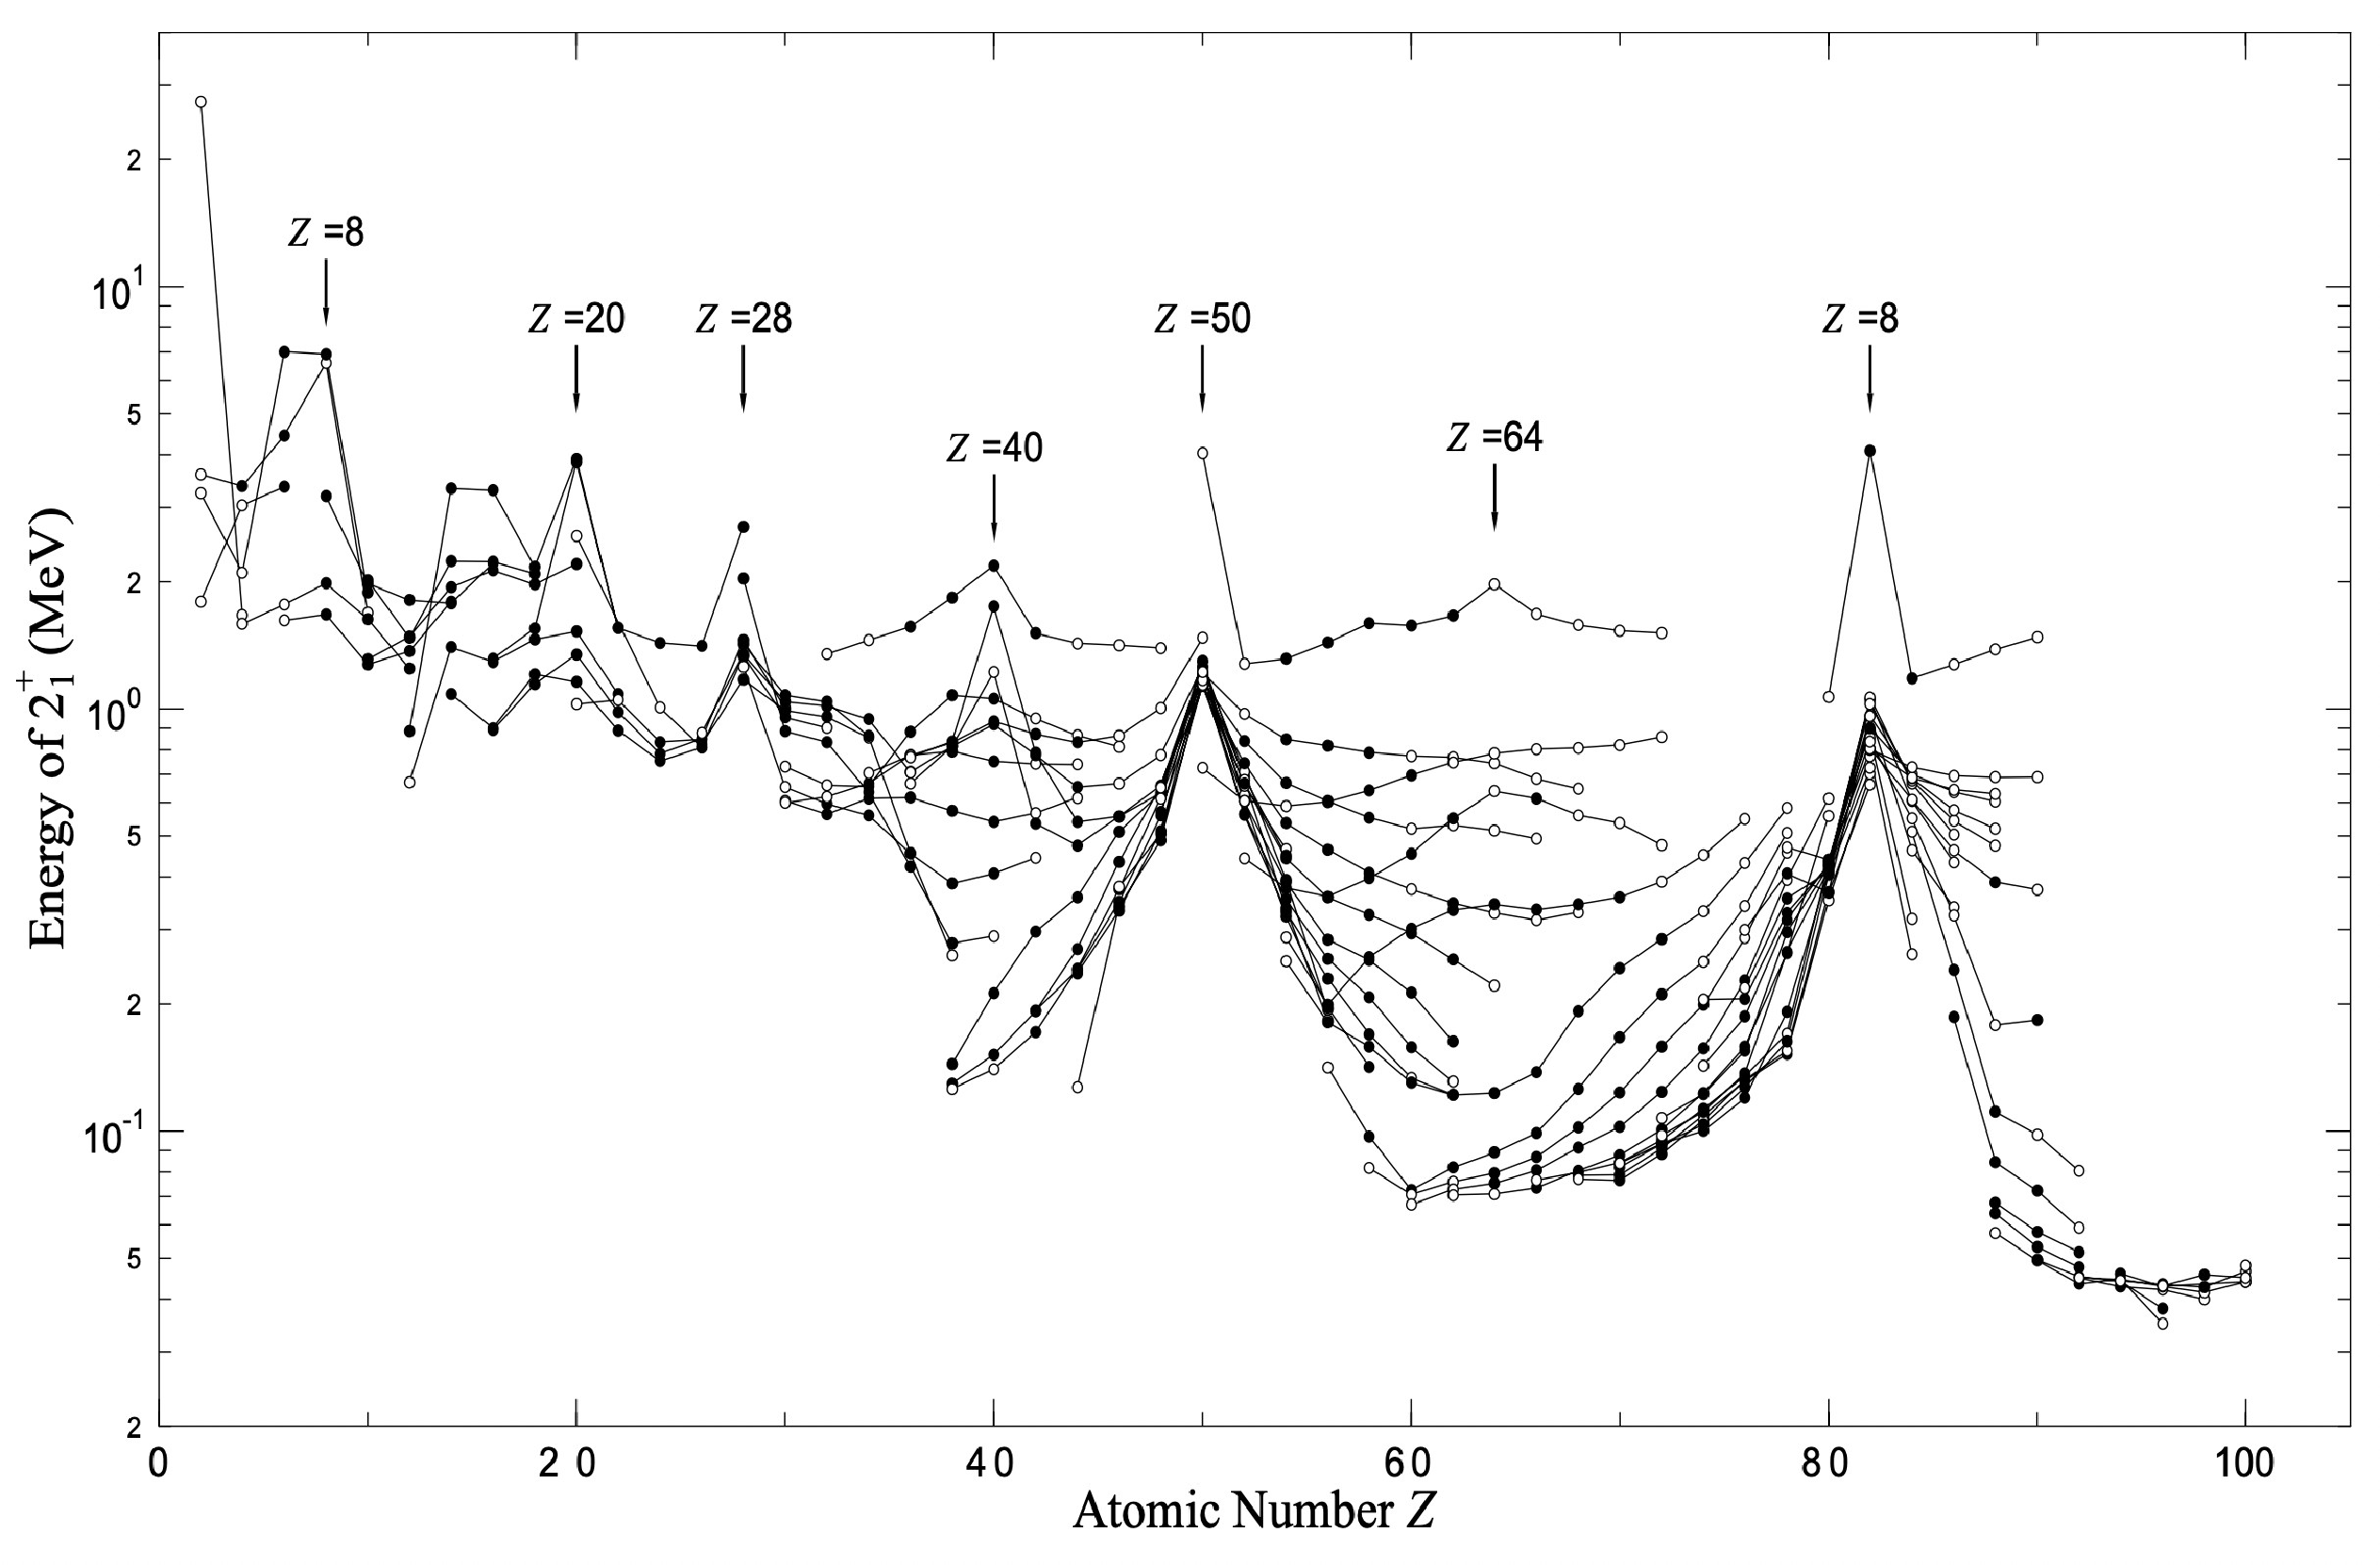
\includegraphics[scale=0.33]{Chapters/Figures/E2plus_proton.pdf}
    \caption{The first excited energy states $2^+$ of nuclei with even $Z$ and $N$ graphically represented with respect to the proton number. Each line represents a set of isotopes. Figure taken from Ref. \cite{matta2017exotic}.}
    \label{e2plus_proton}
\end{figure}

\begin{figure}
    \centering
    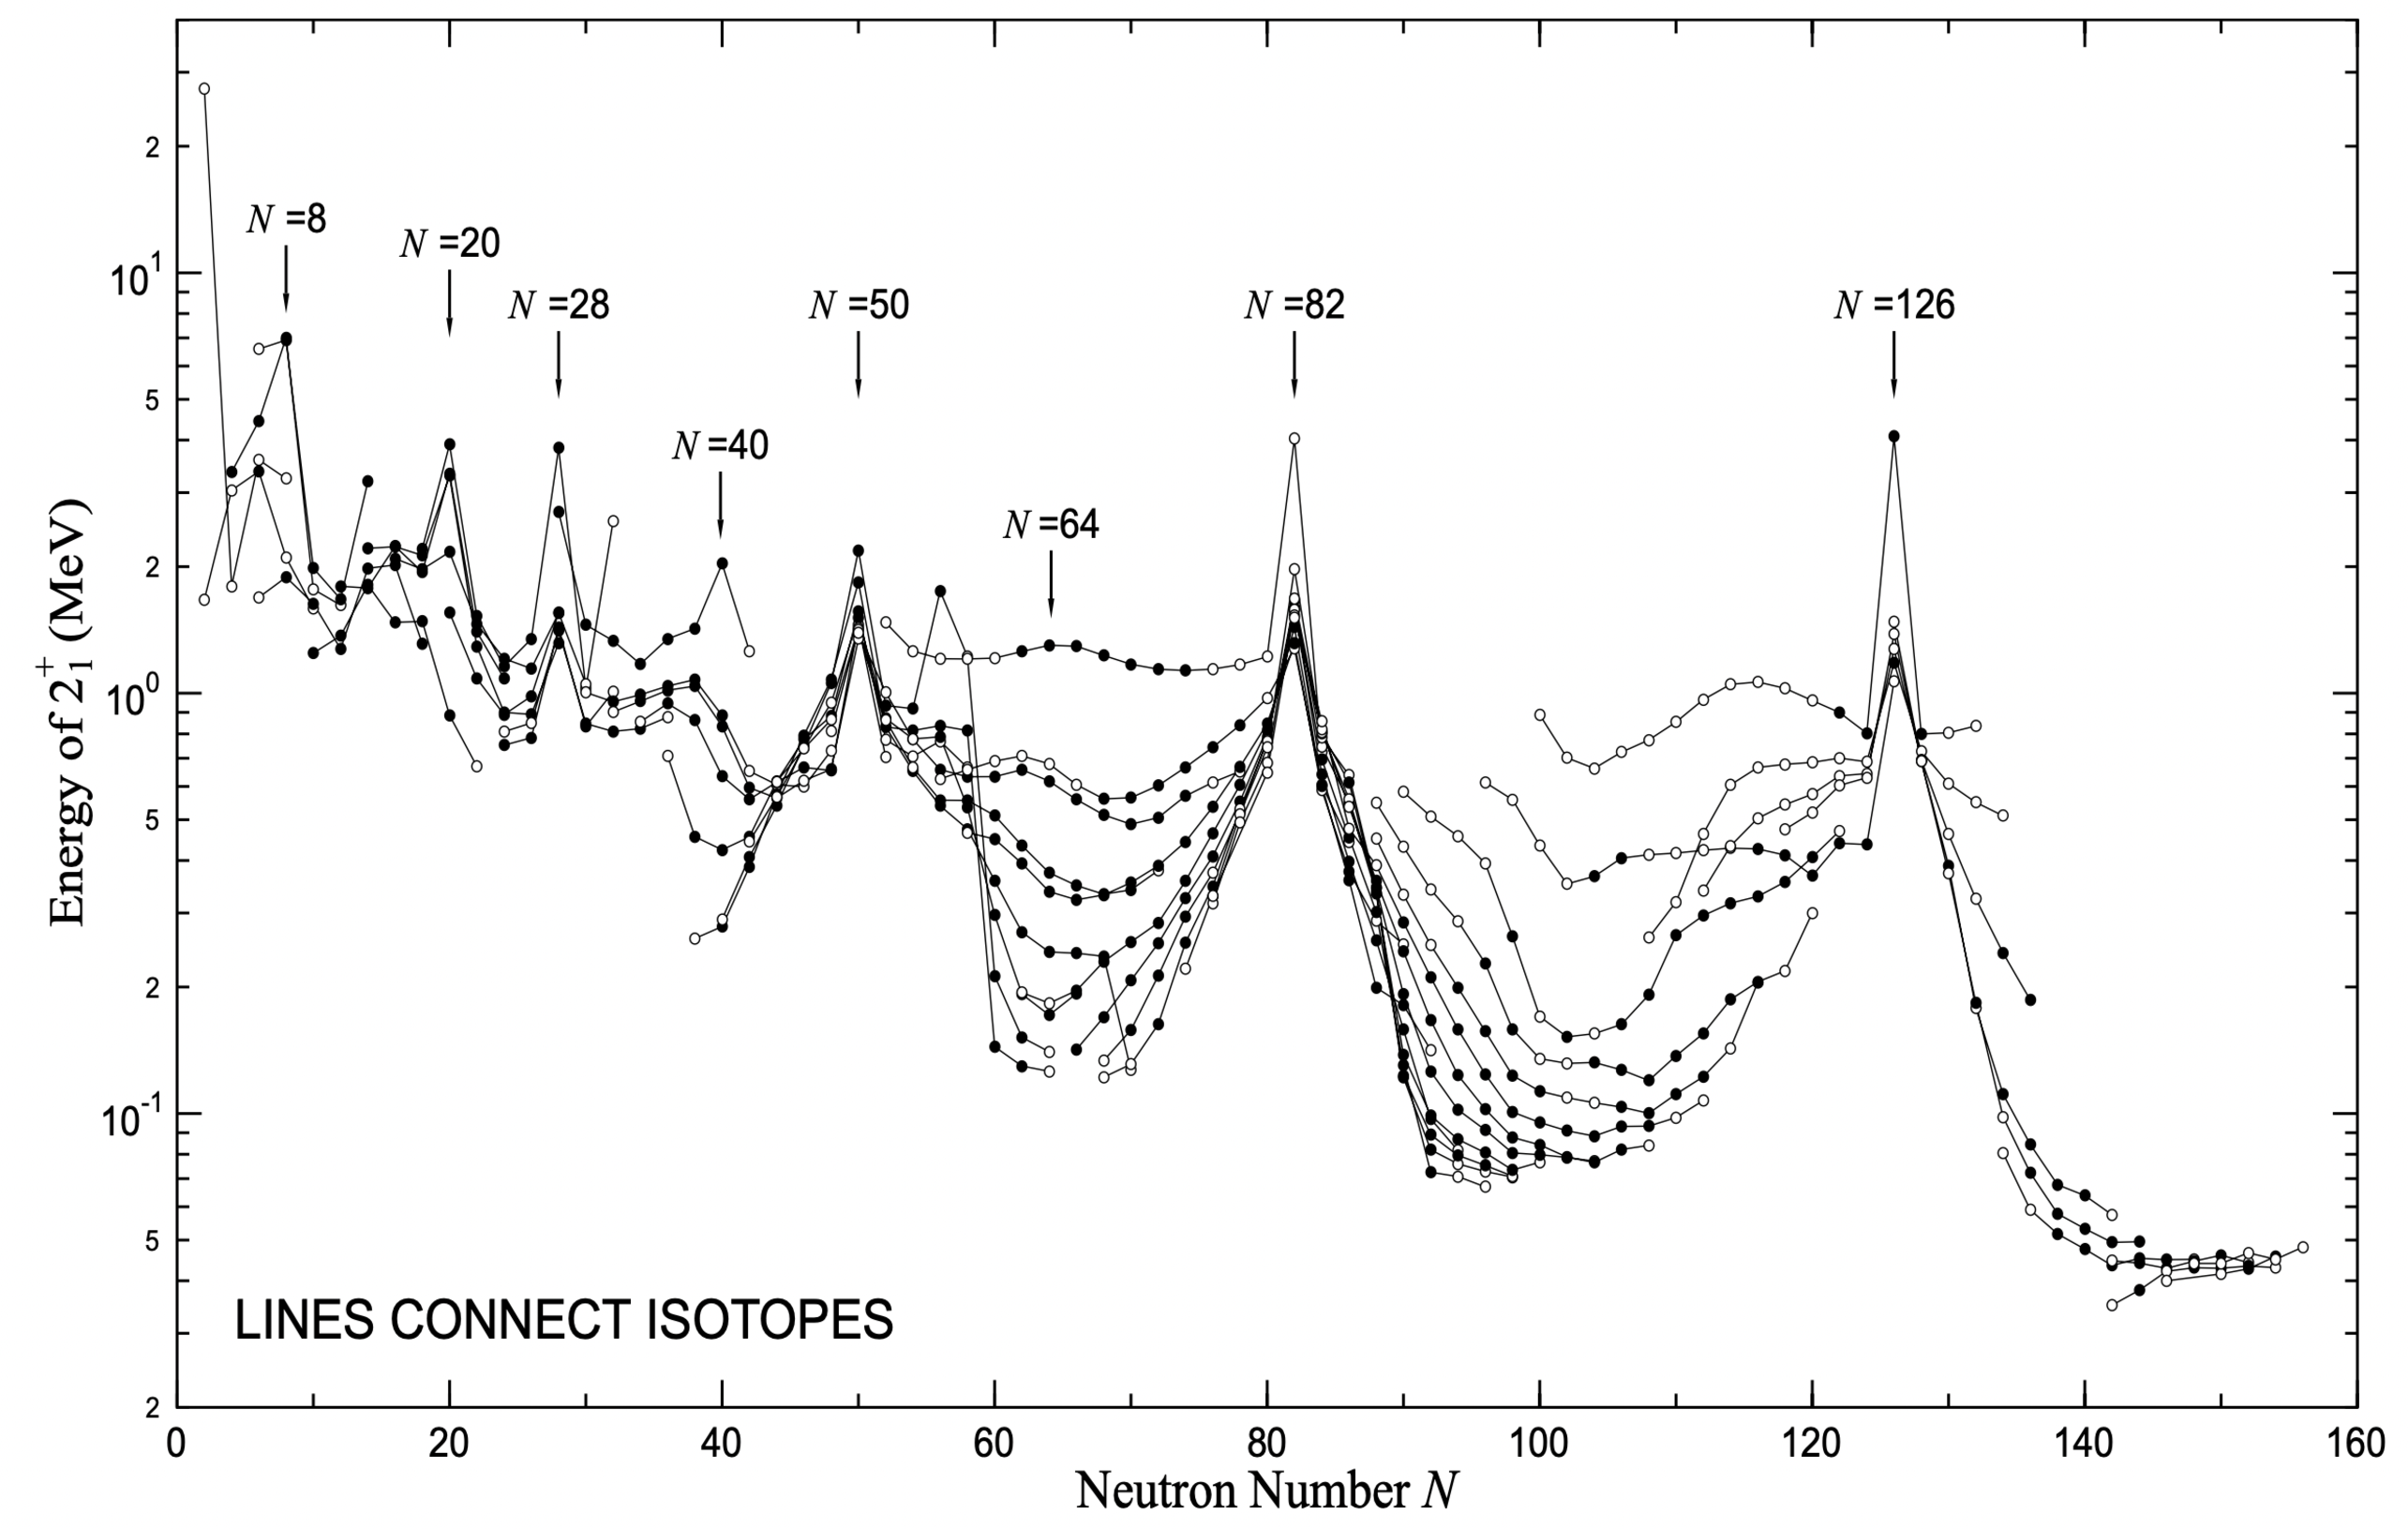
\includegraphics[scale=0.33]{Chapters/Figures/E2plus_neutron.pdf}
    \caption{The first excited energy states $2^+$ of nuclei with even $Z$ and $N$ graphically represented with respect to the neutron number. Each line represents a set of isotopes. Figure taken from Ref. \cite{matta2017exotic}.}
    \label{e2plus_neutron}
\end{figure}

The shell model starts from the basic assumption that the nucleus is a \emph{mean-field potential}, that is a potential for which the motion of a single nucleon is caused by all the other nucleons (the nucleon is moving inside an average potential generated by all the other constituents of the nucleus). Of course, all the nucleons that are under the influence of such a mean field potential occupy the energy levels which correspond to a series of (sub)shells that agree with the Paul exclusion principle. Having a general expression for the potential that properly reproduces all the magic numbers (and the observed nuclear properties) is the main goal.

Since the model starts from the concept of independent (non-interacting) particle motion within an average potential, finding each energy will be equivalent of solving the Schrödinger equation:
\begin{align}
    -\frac{\hbar^2}{2m}\nabla ^2\psi_i(r)+V(r)\psi_i(r)=e_i\psi_i(r)\, 
    \label{schrodinger-single-particle-eq}
\end{align}
where $e_i$ represents the energy (eigenvalue) and $\psi_i$ represents the wave-function (eigenstates), while $V(r)$ is the nuclear potential whose expression must be evaluated.

The choice of $V(r)$ will be dictated by the reproduction of various experimental data (such as nuclear saturation, scattering, nuclear reactions, and so on). For the motion of an independent particle, an obvious first attempt would be the \emph{simple harmonic oscillator} (SHO), which has the known expression:
\begin{align}
    V(r)=\frac{1}{2}m(\omega_i r)^2\ ,
    \label{harmonic-potential}
\end{align}
with $\omega_i$ as the frequency of the basic harmonic-like motion of the particle in the nucleus. With Eq. \ref{harmonic-potential}, the motion of the nucleon has a straightforward expression:
\begin{align}
    \frac{\hbar^2}{2m}\nabla^2\psi_i(r)+\frac{1}{2}m(\omega r)^2\psi_i(r)=e_i\psi_i(r)\ .
\end{align}

This Schrödinger equation has its energy eigenvalues under to form:
\begin{align}
    e_N=\left(N+\frac{3}{2}\right)\hbar\omega\ ,
\end{align}
where $N$ is the number of oscillator quanta which describes each major shell (also called the \emph{principal quantum number}). One should keep in mind that such an expression is typical for a three-dimensional and isotropic harmonic oscillator. The principal quantum number $N$ is furthermore defined as:
\begin{align}
    N=2(n-1)+l\ ,
\end{align}
with $n$ and $l$ being the \emph{radial} quantum number and \emph{orbital angular momentum} quantum number, respectively, taking values $n=1,2,3,\dots$ and $l=0,1,2,\dots,n-1$. In this first approximation, all the levels with the same principal quantum number $N$ are \emph{degenerate}, with a maximal degeneracy given by $2(2l+1)$. However, by using only the SHO term as the expression of $V(r)$, only the first three magic numbers are reproduced, meaning that some additional term(s) might be needed in order to consistently obtain the series of magic numbers.

A next step is to use the fact that the experimentally observed short range of the strong nuclear force: the steepness of the SHO can be corrected with an \emph{attractive} term proportional to $l$-squared. This acts as a centrifugal term which provides an angular momentum barrier, lifting the degeneracy between the levels with the same principal quantum number $N$ and different values for the orbital angular momentum $l$. This SHO+$l^2$ step is still not enough though. The last step is to add a so-called \emph{spin-orbit} coupling term of the form $\vec{l}\cdot\vec{s}$. 
% This last term is enough to reproduce all the magic numbers and the experimentally measured quantities that are relevant to the shell model itself.
This term comes from the consideration that the nucleon-nucleon interaction has a spin dependence, and the potential depends on the intrinsic spin $s$ ($\vec{s}$) and the orbital angular momentum $l$ ($\vec{l}$) of a nucleon. Since $\vec{j}=\vec{l}+\vec{s}$, two possible states emerge from a single value of $l$ (depending on wether $\vec{s}$ is parallel or anti-parallel to $\vec{l}$). The final expression of the terms SHO+$\vec{l}^2$+$\vec{l}\cdot\vec{s}$ will consist in the \emph{Modified Harmonic Oscillator} (HMO).
\begin{align}
    V(r)=\frac{1}{2}(\omega r)^2+B\ \vec{l}^2+A\ \vec{l}\cdot\vec{s}\ .
    \label{modified-harmonic-oscillator-eq}
\end{align}

Since the intrinsic spin of a nucleon is $s=1/2$, for a given value of $l$, there can be two values for the \emph{total angular momentum} (a.m.) $j=l\pm1/2$: one for each spin orientation with respect to the direction of the orbital a.m. Moreover, for each value of $l=0,1,2,3,4,\dots$, there is a similar notation $l=s,p,d,f,g,\dots$, respectively. Regarding the spectroscopic notation, usually, the value of $j$ is considered as a subscript; $nl_j$ (for example $1p_{1/2}$ and $1p_{3/2}$). What it is worth mentioning is that for high enough shells, there can be splittings between $j+1/2$ and $j-1/2$ that are large enough to lower the $j+1/2$ state from one oscillator shell $n$ to one located below $n-1$. These types of levels are called \emph{intruder states} and they have opposite parity $\pi=(-1)^l$ with respect to the shell that these levels will occupy.

Going back to the expression of the $\vec{l}\cdot\vec{s}$ term from Eq. \ref{modified-harmonic-oscillator-eq} and denoting it with $V_{ls}(r)$, it is shown by Casten \cite{casten2000nuclear} that its contribution to the total potential can be regarded as a surface effect. Due to this, its form can be expressed as a function that depends on the radial coordinate as such \cite{casten2000nuclear}:
\begin{align}
    V_{ls}(r)=-a_{ls}\frac{\partial V(r)}{\partial r}\vec{l}\cdot\vec{s}\ ,
\end{align}
where $V(r)$ is the expression for a central potential and $a_{ls}$ is a strength constant.
% Indeed, in the work of Casten \cite{casten2000nuclear}, it is stated that if in the nucleus, the spin-orbit forces were large enough, then there should be an overall preference for nucleons with spins aligned parallel their orbital a.m. other than the opposite alignment, making the nucleons with anti-parallel spins to not be surrounded by an equal number of nucleons with all spin orientations.

Now that an expression for the nuclear potential that is able to reproduce all the magic numbers has been formulated, it is also possible to formulate the total energy of a single-particle within the average potential that is generated by all the other nucleons within the nucleus. Thus, the Hamiltonian of this simple system (the modified oscillator) can be formulated as such:
\begin{align}
    H=\frac{\hbar^2}{2m}\nabla^2+V_\text{SHO}+l^2_\text{term}+\vec{l}\cdot\vec{s}_\text{term}\ , \nonumber\\
    H=\frac{\hbar^2}{2m}\nabla^2+\frac{1}{2}m(\omega r)^2+Bl^2+A\vec{l}\cdot\vec{s}\ .
\end{align}

The evolution from each term in the shell-model potential (that is the first approximation as a SHO, then SHO+$l^2$, and finally SHO+$l^2+\vec{l}\cdot\vec{s}$ or modified oscillator potential) is illustrated in Fig. \ref{energy-levels-mho}, where it can be seen how each extra term introduces a new degeneracy within the energy states, with the complete reproduction of the magic numbers in the third column. Moreover, the \emph{intruder} levels can be observed, where levels with $j=l+1/2$ from a particular $n$ are so low, that they lie below an $n-1$ adjacent level.
\begin{figure}
    \centering
    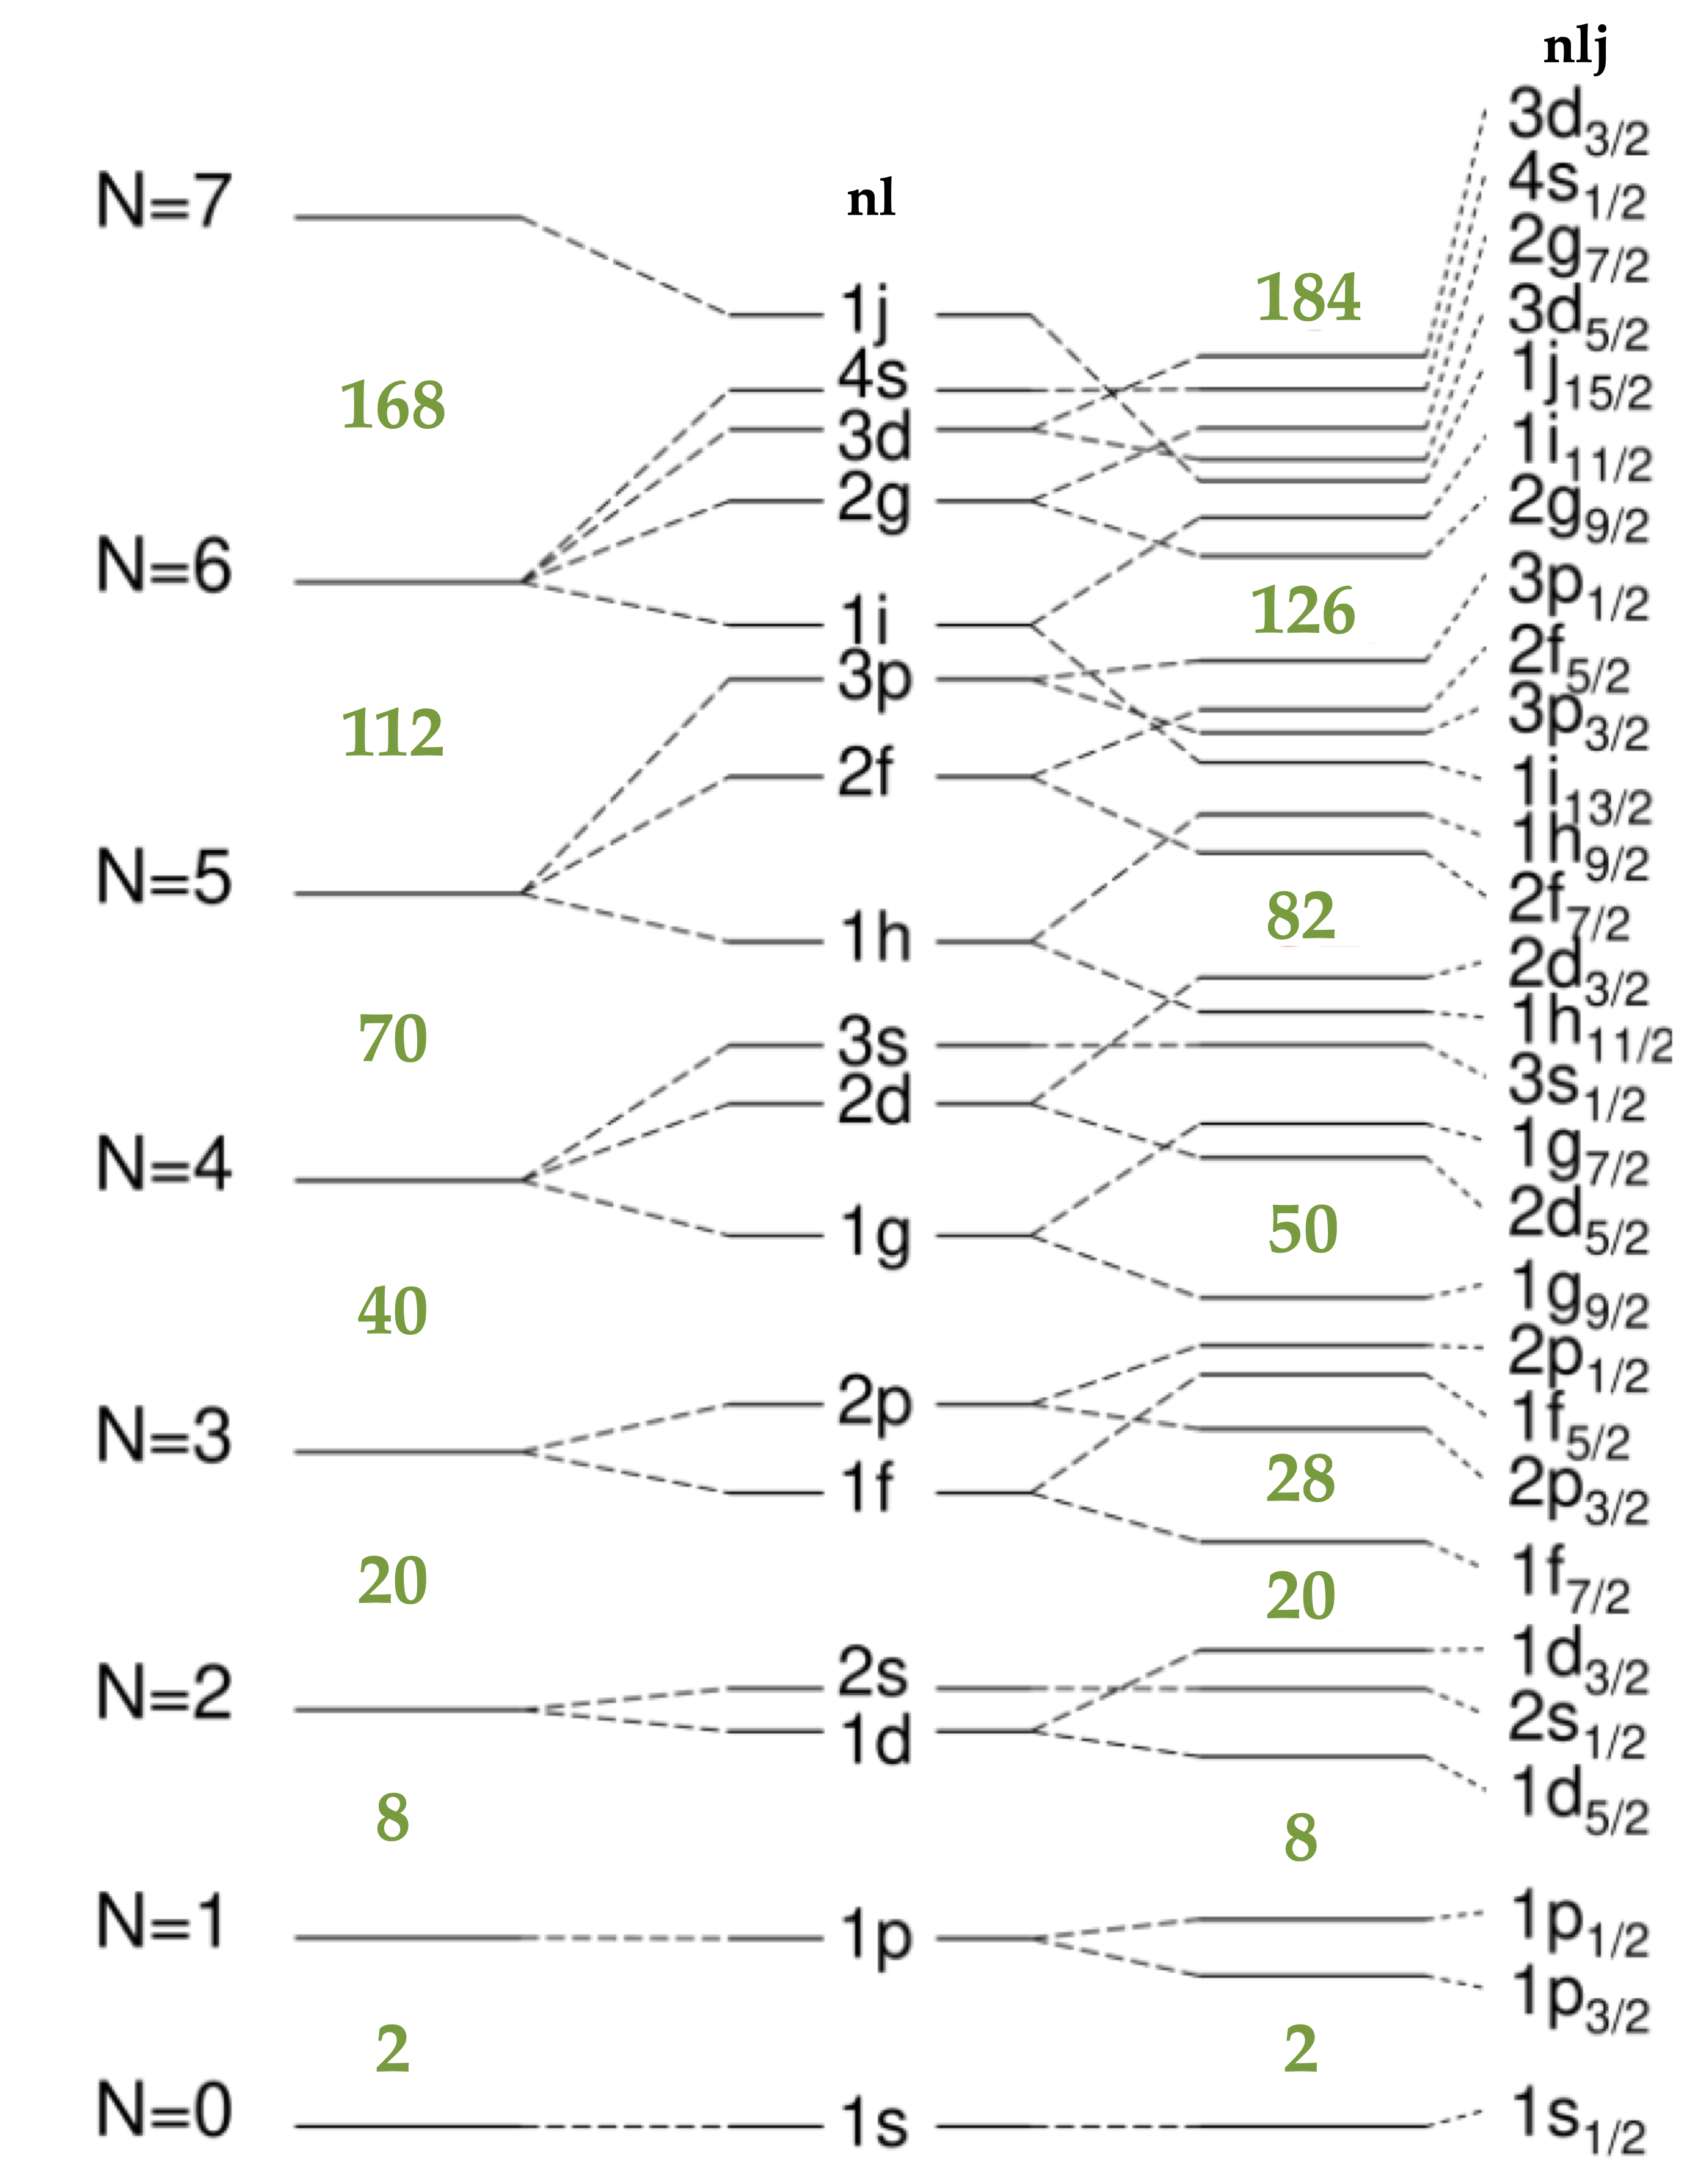
\includegraphics[scale=0.12]{Chapters/Figures/SM_level_scheme.png}
    \caption{The energy levels obtained via calculation of the shell model potential using the simple oscillator (SHO), the SHO amended with a centrifugal term $l^2$, and finally the modified oscillator (MHO) that contains a spin-orbit term. The `correct' magic numbers are the ones in the right-most column. Figure is adapted from Refs. \cite{matta2017exotic},\cite{krane1991introductory}.}
    \label{energy-levels-mho}
\end{figure}

Another, more realistic potential that can be used in order to reproduce the specific shell model calculation is the so-called Woods-Saxon potential. Because of the short-range character of the strong nuclear force, it is safe to assume that this potential should behave in the same manner as the density distribution of the nucleons. Since for medium and heavy nuclei, the Fermi-like functions (distributions) are the ones that best fit the experimentally measured data, this potential should have the following form \cite{woods1954diffuse}:
\begin{align}
    V_\text{ws}=-\frac{V_0}{1+e^{\frac{r-R_0}{a}}}\ .
    \label{woods-saxon-potential}
\end{align}
This mean-field potential contains the terms $V_0$ that represents the depth of the potential ($\approx 50$ MeV, in order to reproduce the experimental separation energies for the nucleons), the surface thickness $a$ (also called the diffuseness parameter, giving information about how fast the potential drops to zero) with a value of approximately $0.5$ fm, while $R_0$ is the nuclear radius with $R_0=r_0A^{1/3}$ and $r_0=1.2$ fm. The nature of this potential is of \emph{central type}, and unfortunately Eq. \ref{woods-saxon-potential} in its pure form is not enough the reproduce the higher magic numbers. As such, the addition of a spin-orbit term, similarly as in the case of MHO potential, is required \cite{martin2017particle}: 
\begin{align}
    V_\text{total}=V_\text{ws}^\text{central}+V_{ls}(r)\vec{l}\cdot\vec{s}\ .
    \label{woods-saxon-so-potential}
\end{align}
The only good quantum numbers in the case of the WS potential are the total a.m. $j$ and the parity $\pi=(-1)^l$.
The expectation value of the spin-orbit term $\vec{l}\cdot\vec{s}$ can be given as:
\begin{align}
    \langle ls \rangle
\end{align}